\subsubsection{Solution updater service}
\textbf{Overview}

The \texttt{SimulationUpdaterService} is a specialized optimization component that iteratively refines simulation models based on result feedback. It serves as the core engine for solution convergence in complex simulation workflows by:

\begin{itemize}
	\item Processing simulation results to derive optimized control vectors
	\item Applying advanced numerical optimization techniques to improve solution quality
	\item Monitoring convergence criteria to determine when solutions have reached acceptable quality
	\item Managing the mapping between domain-specific models and numerical representations
	\item Controlling the iterative optimization process across multiple generations
\end{itemize}

This service is designed for high-performance computing environments where simulations are computationally expensive and optimization requires sophisticated numerical processing. It integrates with larger simulation workflows to provide continuous refinement of model parameters.

\bigskip
\textbf{Architecture}

The \texttt{SimulationUpdaterService} follows a layered architecture pattern that separates concerns between different components of the optimization process.

Key Architectural Principles:
\begin{enumerate}
	\item \textbf{Separation of Concerns}: Each component has a specific responsibility in the optimization workflow.
	
	\item \textbf{Domain-Numerical Translation}: The architecture provides clean translation between domain-specific concepts (control vectors, simulation results) and their numerical representations.
	
	\item \textbf{Encapsulated Optimization}: The optimization engine is abstracted from the business logic of the service.
	
	\item \textbf{Stateful Process Management}: The service maintains state throughout the optimization process while providing a clean API.
	
	\item \textbf{Extensible Design}: The layered architecture allows for replacing components (e.g., optimization algorithms) without affecting the overall system.
\end{enumerate}

\begin{figure}[H]
	\centering
	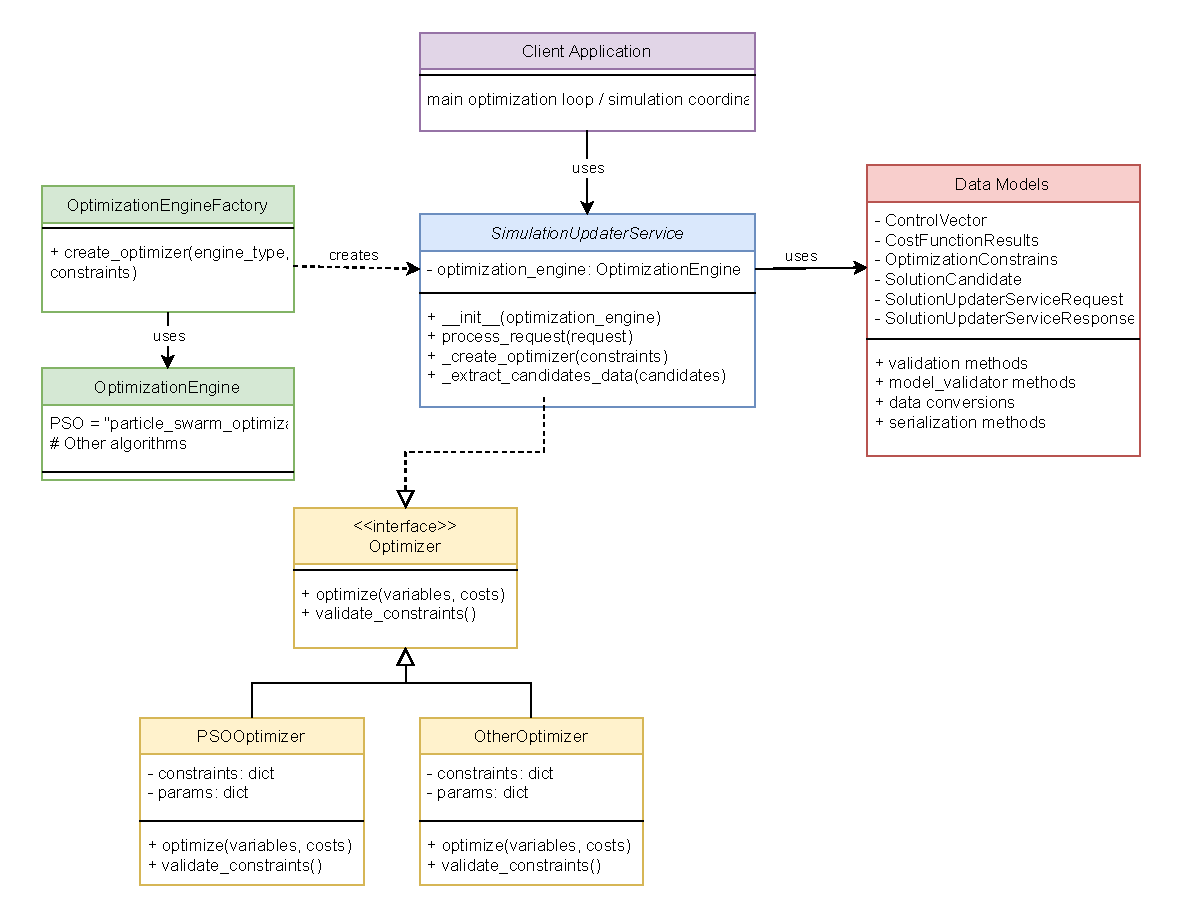
\includegraphics[width=1.0\textwidth]{content/images/SolutionUpdaterUML.pdf}
	\caption{Simulation updater service system UML}
	\label{fig:SolutionUpdaterServiceUML}
\end{figure}

\bigskip
\textbf{System Components}

The \texttt{SimulationUpdaterService} consists of several interconnected components that work together to provide optimization capabilities:

\begin{itemize}
\item \textbf{SimulationUpdaterService}

The main service class that exposes the public API and orchestrates the optimization process.

\textbf{Responsibilities:}
\begin{itemize}
	\item Provide a public interface for clients
	\item Coordinate the optimization workflow
	\item Manage the optimization loop
	\item Check convergence criteria
	\item Return processed results
\end{itemize}

\item \textbf{\_Mapper}

Internal component responsible for translating between domain-specific data structures and numerical representations suitable for optimization algorithms.

\textbf{Responsibilities:}
\begin{itemize}
	\item Convert control vectors to numpy arrays
	\item Convert optimization results back to domain objects
	\item Maintain mappings between domain and numerical representations
	\item Handle variable bounds and constraints
	\item Initialize mapping on first execution
\end{itemize}

\item \textbf{\_MapperState}

Maintains the state of mappings between control vectors, simulation results, and their numerical representations.

\textbf{Responsibilities:}
\begin{itemize}
	\item Store control vector mapping information
	\item Store results mapping information
	\item Track control vector dimensions
	\item Track results dimensions
	\item Store population size information
\end{itemize}

\item \textbf{\_SolutionUpdaterServiceLoopController}

Controls the execution of the optimization loop, tracking progress and termination conditions.

\textbf{Responsibilities:}
\begin{itemize}
	\item Track current generation number
	\item Enforce maximum generation limit
	\item Provide running state information
	\item Offer context manager for loop control
	\item Support early termination
\end{itemize}

\item \textbf{Optimization Engine}

Encapsulated component that implements the mathematical optimization algorithms.

\textbf{Responsibilities:}
\begin{itemize}
	\item Execute numerical optimization operations
	\item Apply optimization techniques to solution arrays
	\item Generate updated solutions based on fitness evaluations
	\item Handle constraints in the optimization process
\end{itemize}

\end{itemize}

\textbf{Public API}

The \texttt{SimulationUpdaterService} exposes a minimal yet powerful public API that provides access to its optimization capabilities. This section details each public method, its parameters, return values, and implementation details.

\begin{itemize}
	\item SimulationUpdaterService Constructor
	
	Initializes a new instance of the \texttt{SimulationUpdaterService} class. This constructor sets up the internal components required for the optimization process, including the mapper, optimization engine, and loop controller.
	
	\textbf{Implementation Details}
	
	The constructor performs the following initialization steps:
	\begin{itemize}
		\item Creates a new instance of the \texttt{\_Mapper} class for domain-numerical translation
		\item Initializes the optimization engine with default configuration
		\item Sets up a logger for diagnostic information
		\item Creates a \texttt{\_SolutionUpdaterServiceLoopController} instance to manage the optimization loop
	\end{itemize}

	\textbf{Error Handling}
	\begin{itemize}
		\item Any exceptions during initialization are allowed to propagate, as they indicate critical setup problems that should prevent service creation
		\item If dependencies are not available or incorrectly configured, appropriate import or initialization errors will be raised
	\end{itemize}

	\item \csignature{process\_request(self, request)}
	
	Processes an optimization request by iteratively updating the solution based on simulation results. This method represents the core functionality of the service, orchestrating the complete optimization workflow from initial population to converged solutions.
	
	\textbf{Implementation Details}
	
	The method implements a complete optimization step:
	\begin{enumerate}
		\item Validates the input request for required fields and data consistency
		\item Initializes the mapper with the domain-specific structure of control vectors and results
		\item Converts the domain objects to numerical arrays suitable for optimization
		\item Sets up the optimization loop with appropriate constraints and parameters
		\item Executes the optimization process for multiple generations until convergence or maximum generations
		\item Periodically checks for convergence based on defined criteria
		\item Translates the optimized numerical results back to domain-specific control vectors
		\item Prepares and returns a comprehensive response with the optimization results
	\end{enumerate}

	\textbf{Error Handling}
	\begin{itemize}
		\item \textbf{ValueError}: Raised if the request is missing required fields or contains inconsistent data
		\begin{itemize}
			\item Missing initial population or simulation results
			\item Mismatch between population size and results size
			\item Invalid configuration parameters (negative max generations, etc.)
		\end{itemize}
		
		\item \textbf{TypeError}: Raised if the data types in the request are incompatible with the optimization process
		\begin{itemize}
			\item Non-numeric values in control vectors or results
			\item Incompatible constraint formats
		\end{itemize}
		
		\item \textbf{RuntimeError}: Raised if the optimization process encounters an unrecoverable error
		\begin{itemize}
			\item Optimization algorithm failure
			\item Numerical stability issues
			\item Resource limitations
		\end{itemize}
		
		\item \textbf{Exception Handling}: The method includes comprehensive exception handling to:
		\begin{itemize}
			\item Log detailed diagnostic information
			\item Provide informative error messages
			\item Clean up resources in case of failures
			\item Convert low-level numerical exceptions to domain-appropriate exceptions
		\end{itemize}
	\end{itemize}

	\item \textbf{Loop controller}
	
	A property that provides access to the optimization loop controller. The loop controller exposes information about the optimization process state and provides control over the execution of the optimization loop:
	
	\begin{itemize}
		\item Maintains state about the current generation number
		\item Tracks whether the optimization loop is currently running
		\item Provides a context manager for the optimization loop execution
		\item Enforces maximum generation constraints
		\item Supports early termination of the optimization process
	\end{itemize}
	
	The controller is typically used internally by the \texttt{process\_request} method, but is exposed as a public property to allow advanced clients to access detailed state information or implement custom loop control if needed.
	
\end{itemize}

\textbf{Data Models Schema}

The \texttt{SimulationUpdaterService} uses a structured set of data models to represent optimization problems, solution candidates, and constraints. This section details the schemas of these models and their relationships.

\begin{lstlisting}[language=Python, caption={OptimizationEngine enumeration definition}]
	class OptimizationEngine(Enum):
	"""Enumeration of available optimization algorithms."""
	
	PSO = "particle_swarm_optimization"
	# Other algorithm types can be added here
\end{lstlisting}

\textbf{Description:}
The \texttt{OptimizationEngine} enumeration defines the available optimization algorithms that can be used by the service. Currently, it includes Particle Swarm Optimization (PSO), but the system is designed to be extensible with additional algorithms in the future.

\begin{lstlisting}[language=Python, caption={ControlVector model definition}]
	from pydantic import BaseModel, Field
	
	class ControlVector(BaseModel, extra="forbid"):
	"""Represents a collection of optimization variables."""
	
	items: Dict[str, float]
\end{lstlisting}

\textbf{Description:}
The \texttt{ControlVector} model represents the input parameters that control a simulation. Each item in the dictionary corresponds to a single optimization variable (e.g., "pressure", "temperature") with its associated value. The optimization process will aim to find optimal values for these variables.

\textbf{Validation Requirements:}
\begin{itemize}
	\item The items dictionary must not be empty
	\item All keys must be strings representing variable names
	\item All values must be floating-point numbers within valid numerical ranges
\end{itemize}

\begin{lstlisting}[language=Python, caption={CostFunctionResults model definition}]
	from pydantic import BaseModel, Field
	
	class CostFunctionResults(BaseModel, extra="forbid"):
	"""Stores the results of cost function calculations."""
	
	values: Dict[str, float]
\end{lstlisting}

\textbf{Description:}
The \texttt{CostFunctionResults} model stores the output metrics from simulation runs. Each item in the dictionary represents a cost function (e.g., "heat\_transfer", "flow\_rate") with its calculated value. These values are used to evaluate how good a particular solution is and guide the optimization process.

\textbf{Validation Requirements:}
\begin{itemize}
	\item The values dictionary must not be empty
	\item All keys must be strings representing cost function names
	\item All values must be floating-point numbers
\end{itemize}

\begin{lstlisting}[language=Python, caption={OptimizationConstrains model with validation logic}]
	from pydantic import BaseModel, Field, model_validator
	
	class OptimizationConstrains(BaseModel, extra="forbid"):
	"""Defines the constraints for the optimization variables."""
	
	boundaries: Dict[str, Tuple[float, float]]
	
	@model_validator(mode='after')
	def validate_lower_bound_is_less_than_upper_bound(self) -> 'OptimizationConstrains':
	"""Validates that lower bounds are less than upper bounds."""
		for var_name, (lower, upper) in self.boundaries.items():
			if lower >= upper:
				raise ValueError(
				f"Lower bound must be less than upper bound for {var_name}. "
				f"Got: lower={lower}, upper={upper}"
		)
	return self
\end{lstlisting}


\textbf{Description:}
The \texttt{OptimizationConstrains} model defines the valid ranges for optimization variables. Each entry in the boundaries dictionary maps a variable name to its allowed range as a tuple of (lower\_bound, upper\_bound). The optimization process will ensure that all solutions stay within these boundaries.

\textbf{Validation Requirements:}
\begin{itemize}
	\item For each variable, the lower bound must be strictly less than the upper bound
	\item All boundary values must be valid floating-point numbers
	\item Variable names in boundaries should match those used in ControlVector
\end{itemize}

\begin{lstlisting}[language=Python, caption={SolutionCandidate model definition}]
	from pydantic import BaseModel, Field
	
	class SolutionCandidate(BaseModel, extra="forbid"):
	"""Represents a complete solution with inputs and results."""
	
	control_vector: ControlVector
	cost_function_results: CostFunctionResults
\end{lstlisting}

\textbf{Description:}
The \texttt{SolutionCandidate} model represents a complete solution in the optimization process, pairing a specific set of input parameters with their resulting simulation outputs. Each candidate represents one point in the solution space, and the optimization process evaluates and compares candidates to find better solutions.

\textbf{Validation Requirements:}
\begin{itemize}
	\item Both control\_vector and cost\_function\_results must be provided
	\item The control\_vector must be a valid ControlVector instance
	\item The cost\_function\_results must be a valid CostFunctionResults instance
\end{itemize}

\begin{lstlisting}[language=Python, caption={SolutionUpdaterServiceRequest model with complex validation logic}]
	from pydantic import BaseModel, Field, model_validator
	from typing import List, Optional
	
	class SolutionUpdaterServiceRequest(BaseModel, extra="forbid"):
	"""The complete request for optimization."""
	
	solution_candidates: List[SolutionCandidate]
	optimization_constraints: Optional[OptimizationConstrains] = None
	
	@model_validator(mode='after')
	def validate_solution_candidates_contain_the_same_cost_functions(self) -> 'SolutionUpdaterServiceRequest':
	"""Validates that all solution candidates use the same set of cost functions."""
	if not self.solution_candidates:
	return self
	
	reference_candidate = self.solution_candidates[0]
	reference_cost_functions = set(reference_candidate.cost_function_results.values.keys())
	
	for idx, candidate in enumerate(self.solution_candidates[1:], start=1):
	candidate_cost_functions = set(candidate.cost_function_results.values.keys())
	if reference_cost_functions != candidate_cost_functions:
	raise ValueError(
	f"All solution candidates must contain the same cost functions. "
	f"Mismatch at candidate {idx}. "
	f"Expected: {reference_cost_functions}, "
	f"Got: {candidate_cost_functions}"
	)
	return self
	
	@model_validator(mode='after')
	def validate_solution_candidates_contain_the_same_optimization_variables(self) -> 'SolutionUpdaterServiceRequest':
	"""Validates that all solution candidates use the same set of optimization variables."""
	if not self.solution_candidates:
	return self
	
	reference_candidate = self.solution_candidates[0]
	reference_variables = set(reference_candidate.control_vector.items.keys())
	
	for idx, candidate in enumerate(self.solution_candidates[1:], start=1):
	candidate_variables = set(candidate.control_vector.items.keys())
	if reference_variables != candidate_variables:
	raise ValueError(
	f"All solution candidates must contain the same optimization variables. "
	f"Mismatch at candidate {idx}. "
	f"Expected: {reference_variables}, "
	f"Got: {candidate_variables}"
	)
	return self
	
	@model_validator(mode='after')
	def validate_optimization_boundaries_contain_the_same_optimization_variables(self) -> 'SolutionUpdaterServiceRequest':
	"""Validates that optimization boundaries match the variables used in solutions."""
	if not self.solution_candidates or not self.optimization_constraints:
	return self
	
	reference_candidate = self.solution_candidates[0]
	reference_variables = set(reference_candidate.control_vector.items.keys())
	boundary_variables = set(self.optimization_constraints.boundaries.keys())
	
	if reference_variables != boundary_variables:
	raise ValueError(
	f"Optimization boundaries must contain the same variables as solution candidates. "
	f"Solution variables: {reference_variables}, "
	f"Boundary variables: {boundary_variables}"
	)
	return self
	
	@model_validator(mode='after')
	def reorder_solution_candidates_optimization_variables_and_cost_functions(self) -> 'SolutionUpdaterServiceRequest':
	"""Reorders variables and cost functions for consistent processing."""
	# Implementation handles consistency of ordering across solution candidates
	return self
\end{lstlisting}

\textbf{Description:}
The \texttt{SolutionUpdaterServiceRequest} model represents a complete request to the optimization service. It contains the initial population of solution candidates and optional constraints. The service processes this request to generate an optimized set of solutions.

The model includes several validation methods to ensure consistency across the solution candidates:
\begin{itemize}
	\item Ensures all candidates use the same cost functions
	\item Ensures all candidates use the same optimization variables
	\item Verifies that optimization boundaries match the variables used
	\item Reorders variables and cost functions for consistent processing
\end{itemize}

\textbf{Validation Requirements:}
\begin{itemize}
	\item Must contain at least one solution candidate
	\item All solution candidates must use the same set of cost function names
	\item All solution candidates must use the same set of optimization variable names
	\item If constraints are provided, they must cover the same variable names
\end{itemize}







\bigskip
\textbf{Detailed Workflow}
The optimization process within the \texttt{SimulationUpdaterService} follows a systematic workflow that translates domain-specific inputs into optimized outputs through several processing stages.

\begin{enumerate}
	
\item Initialization Phase

\begin{enumerate}
	\item \textbf{Request Validation}: The service validates the incoming request to ensure it contains the required data.
	
	\item \textbf{Mapper Initialization}: On first execution, the mapper analyzes the structure of control vectors and results to create appropriate mappings.
	
	\item \textbf{State Preparation}: The service initializes the optimization state, including:
	\begin{itemize}
		\item Population arrays
		\item Results arrays
		\item Constraint definitions
		\item Variable bounds
		\item Generation counters
	\end{itemize}
	
	\item \textbf{Engine Configuration}: The optimization engine is configured with appropriate parameters for the specific problem.
\end{enumerate}

\item Optimization Step

The main optimization step executes the following steps for each generation:

\begin{enumerate}
	\item \textbf{Population Conversion}: Control vectors are converted to numerical arrays using the mapper.
	
	\item \textbf{Fitness Evaluation}: The fitness of each solution is calculated based on simulation results.
	
	\item \textbf{Selection}: The most promising individuals are selected for producing the next generation.
	
	\item \textbf{Variation Operations}: The optimization engine applies:
	\begin{itemize}
		\item Crossover between selected individuals
		\item Mutation to maintain diversity
		\item Constraint handling to ensure valid solutions
	\end{itemize}
	
	\item \textbf{Population Update}: The new generation replaces the previous one.
	
	\item \textbf{Convergence Check}: The service evaluates whether the optimization has converged using:
	\begin{itemize}
		\item Change in objective function values
		\item Population diversity metrics
		\item Constraint satisfaction levels
		\item Stability of the best solution
	\end{itemize}
	
	\item \textbf{Loop Control}: The controller updates generation counters and checks for termination conditions.
\end{enumerate}

\item Finalization Phase

After the optimization step completes (either through convergence or reaching maximum generations):

\begin{enumerate}
	\item \textbf{Result Translation}: The final numerical solutions are converted back to domain-specific control vectors.
	
	\item \textbf{Metrics Compilation}: Convergence metrics and optimization statistics are compiled.
	
	\item \textbf{Response Preparation}: A structured response is created containing:
	\begin{itemize}
		\item Optimized control vectors
		\item Convergence metrics and history
		\item Termination reason
		\item Generation statistics
	\end{itemize}
	
	\item \textbf{Resource Cleanup}: Any temporary resources used during optimization are released.
\end{enumerate}

\end{enumerate}